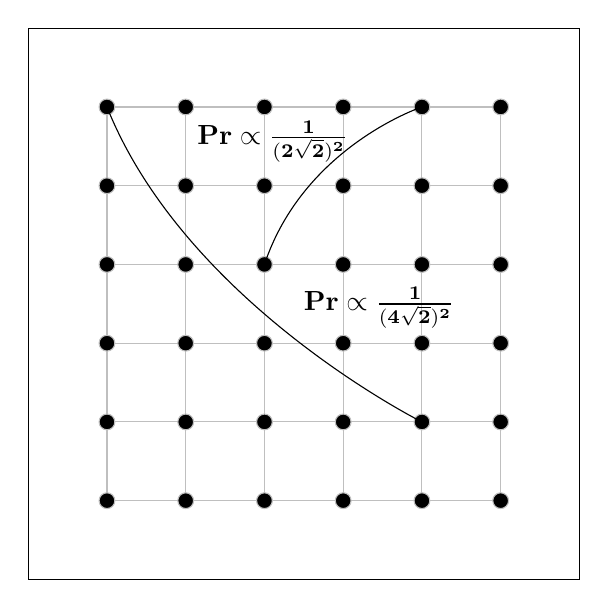
\begin{tikzpicture}[]
    % Grid
    \draw[clip] (-1,-1) rectangle (6,6);
    \draw[step=1,color=lightgray] (0,0) grid (5,5);
    \foreach \xpos in {0, 1, 2, 3, 4, 5}
    {
      \foreach \ypos in {0, 1, 2, 3, 4, 5}
      {
      \draw [color=lightgray,fill=black,opacity=1.0] (\xpos,\ypos) circle (0.1);
      };
    };

    % Draw some long range edges
   \draw (2,3)  .. controls (2.5,4.5) and (4,5) .. node [left] {$\mathbf{Pr \propto \frac{1}{(2\sqrt{2})^2}}$} (4,5);
   \draw (0,5)  .. controls (1.0,2.5) and (4,1) ..  node [above right] {$\mathbf{Pr \propto \frac{1}{(4\sqrt{2})^2}}$} (4,1);

\end{tikzpicture}